\documentclass[11pt]{article}
\usepackage[letterpaper,landscape,margin=0.65in]{geometry}
\usepackage{booktabs,graphicx}
\setlength{\parindent}{0pt}
\setlength{\parskip}{6pt}
\begin{document}
\begin{center}\Large\textbf{Risk-survey responses across four group CCEI-CEIV categories}\end{center}
\textbf{Sample.} All available risk-survey responses from both waves, with no restriction on the members' risk-preference
gap. Classification matches Figure 6: indices within $10^{-9}$ of one count as one. CEIV classifications agree at both
supplied numerical bounds. The 1,304 pair-wave observations supply 2,608 respondent-waves; one respondent has missing
answers to all three questions, leaving 2,607 responses for each question.

\begin{center}\small\begin{tabular}{clrrrrr}\toprule
Category & Group outcomes & Pair-waves & Respondents & Cooperation & Similarity & ``Both''\\
& & & with answers & Mean (1--5) & Mean (1--4) & Share (\%)\\\midrule
1 & CCEI$<1$, CEIV$<1$ & 415 & 830 & 4.380 & 2.963 & 67.5\\
2 & CCEI$=1$, CEIV$<1$ & 117 & 234 & 4.423 & 3.051 & 68.8\\
3 & CCEI$<1$, CEIV$=1$ & 300 & 600 & 4.368 & 3.047 & 68.5\\
4 & CCEI$=1$, CEIV$=1$ & 472 & 943 & 4.512 & 3.232 & 66.3\\
\bottomrule\end{tabular}\end{center}
\textbf{Relevant contrast: category 4 minus category 3.} Both categories have CEIV$=1$;
they differ in whether group CCEI also equals one. This comparison does not hold other pair characteristics fixed.
\begin{center}\small
\begin{tabular}{lrrr}\toprule
Survey measure & Difference & 95\% confidence interval & $p$\\\midrule
Cooperation score & 0.144 & [0.026, 0.262] & 0.018\\
Similarity score & 0.186 & [0.078, 0.293] & $<0.001$\\
Both suggestions reflected (percentage points) & -2.222 & [-7.599, 3.155] & 0.412\\
\bottomrule\end{tabular}\end{center}

\small
\textbf{Reading the pattern.} Groups with both indices equal to one report somewhat more cooperation and greater
similarity to hypothetical own choices. They do not report ``Both'' suggestions more often than CEIV-only groups.
These findings support perceived alignment more directly than a particular method of preference aggregation.
The survey cannot identify a conversation about preferences, stable weights, or turn-taking; group CCEI and CEIV do
not identify those processes either.

\textit{Inference:} Descriptive, unadjusted comparisons with standard errors clustered by 64 classes. Ordinal means assume
equal spacing between coded responses and are supplemented by full response distributions. No mean is assigned to the
nominal whose-suggestions question. Reported $p$-values are exploratory and have no multiple-testing adjustment.
\clearpage
\begin{center}\Large\textbf{Reported cooperation}\end{center}
\begin{center}
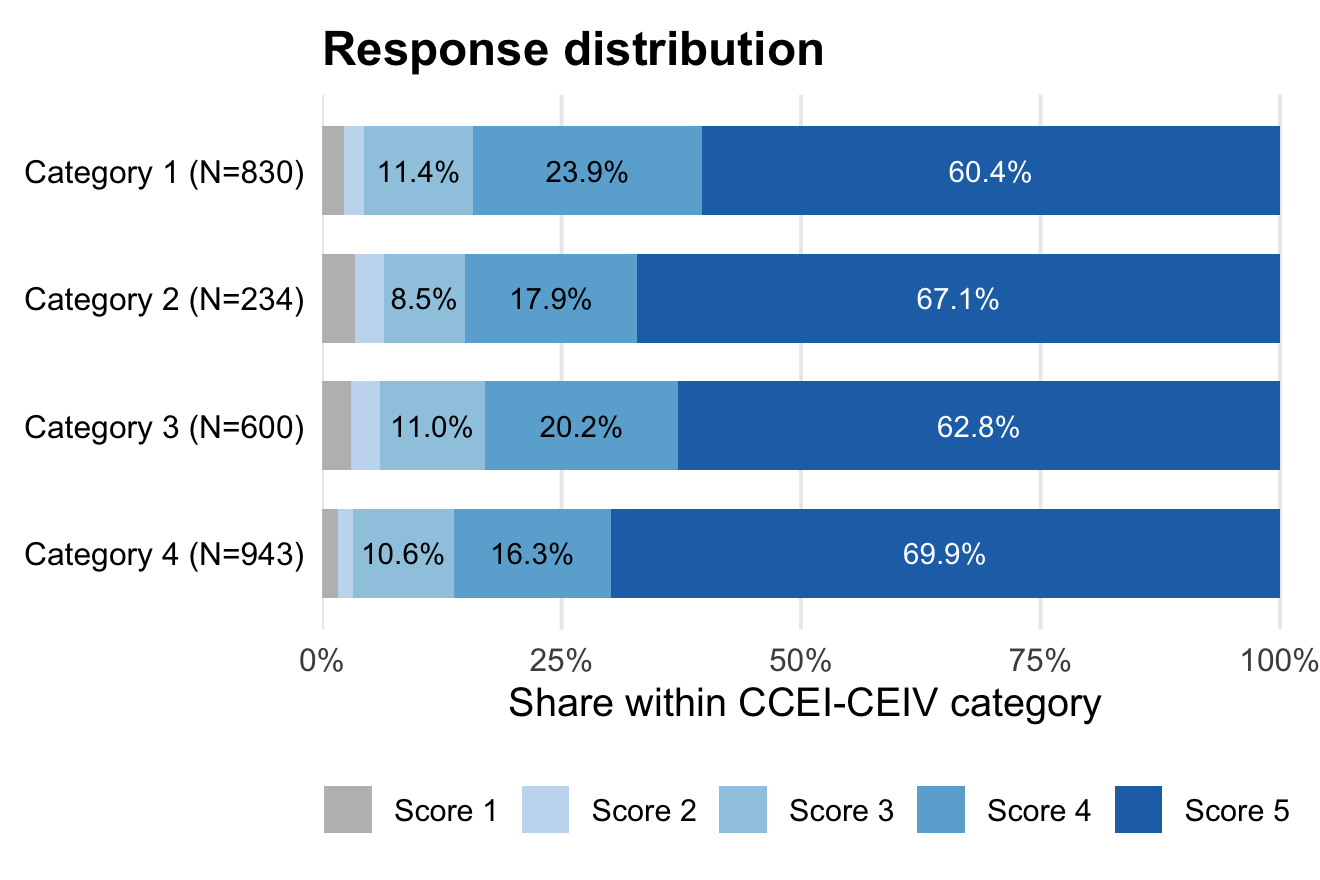
\includegraphics[width=0.595\textwidth]{cooperation_distribution.png}
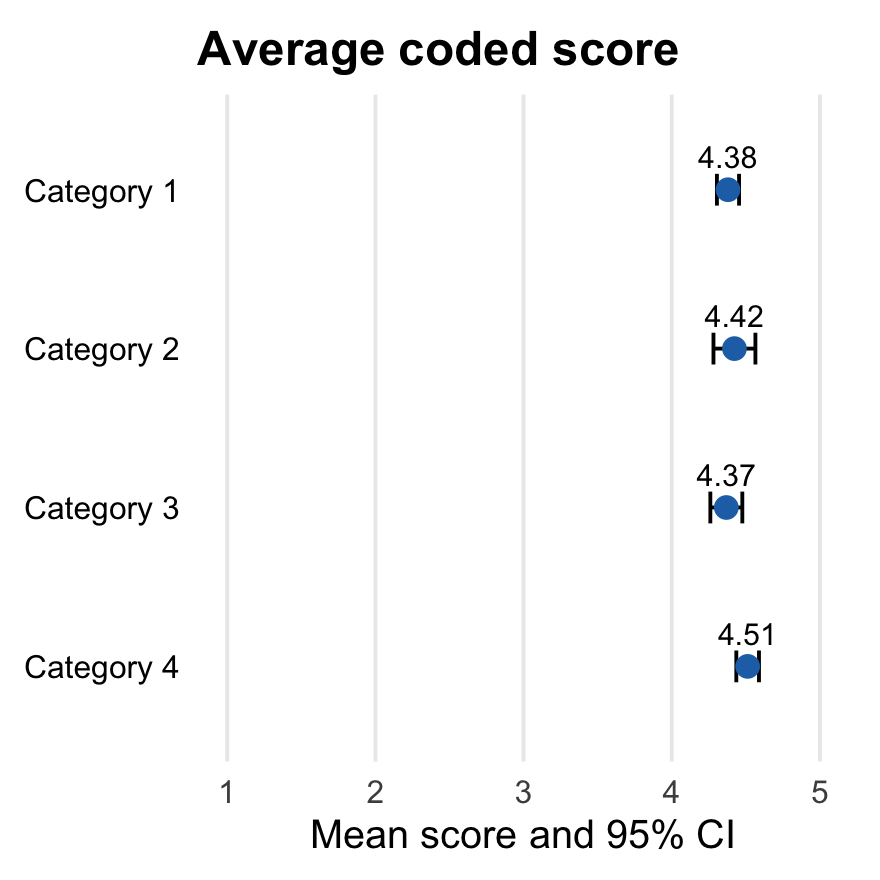
\includegraphics[width=0.395\textwidth]{cooperation_mean.png}
\end{center}
\small
Cooperation uses coded scores 1 to 5, with higher scores indicating greater cooperation. Exact original wording and answer anchors have not been recovered and are not reconstructed here.

\begin{center}\begin{tabular}{clrrrrr}\toprule
Category & Group outcomes & 1 & 2 & 3 & 4 & 5\\\midrule
1 & CCEI$<1$, CEIV$<1$ & 2.3 & 2.0 & 11.4 & 23.9 & 60.4\\
2 & CCEI$=1$, CEIV$<1$ & 3.4 & 3.0 & 8.5 & 17.9 & 67.1\\
3 & CCEI$<1$, CEIV$=1$ & 3.0 & 3.0 & 11.0 & 20.2 & 62.8\\
4 & CCEI$=1$, CEIV$=1$ & 1.7 & 1.5 & 10.6 & 16.3 & 69.9\\
\bottomrule\end{tabular}\end{center}
\textit{Notes:} Table entries are percentages within each group category. Response counts are 830, 234, 600, 943. Category 4 has one missing respondent; all other responses are observed. Joint class-clustered tests of equal response distributions: all four categories, $p=0.008$; categories 4 and 3, $p=0.044$. Tests use stacked linear probability models for all but one response indicator, with unrestricted category-by-response means.
Category 4 minus category 3 in mean score: 0.144 ($p=0.018$). Mean-score intervals are 95\% t intervals using class-clustered standard errors.
\clearpage
\begin{center}\Large\textbf{Similarity of hypothetical own choices}\end{center}
\begin{center}
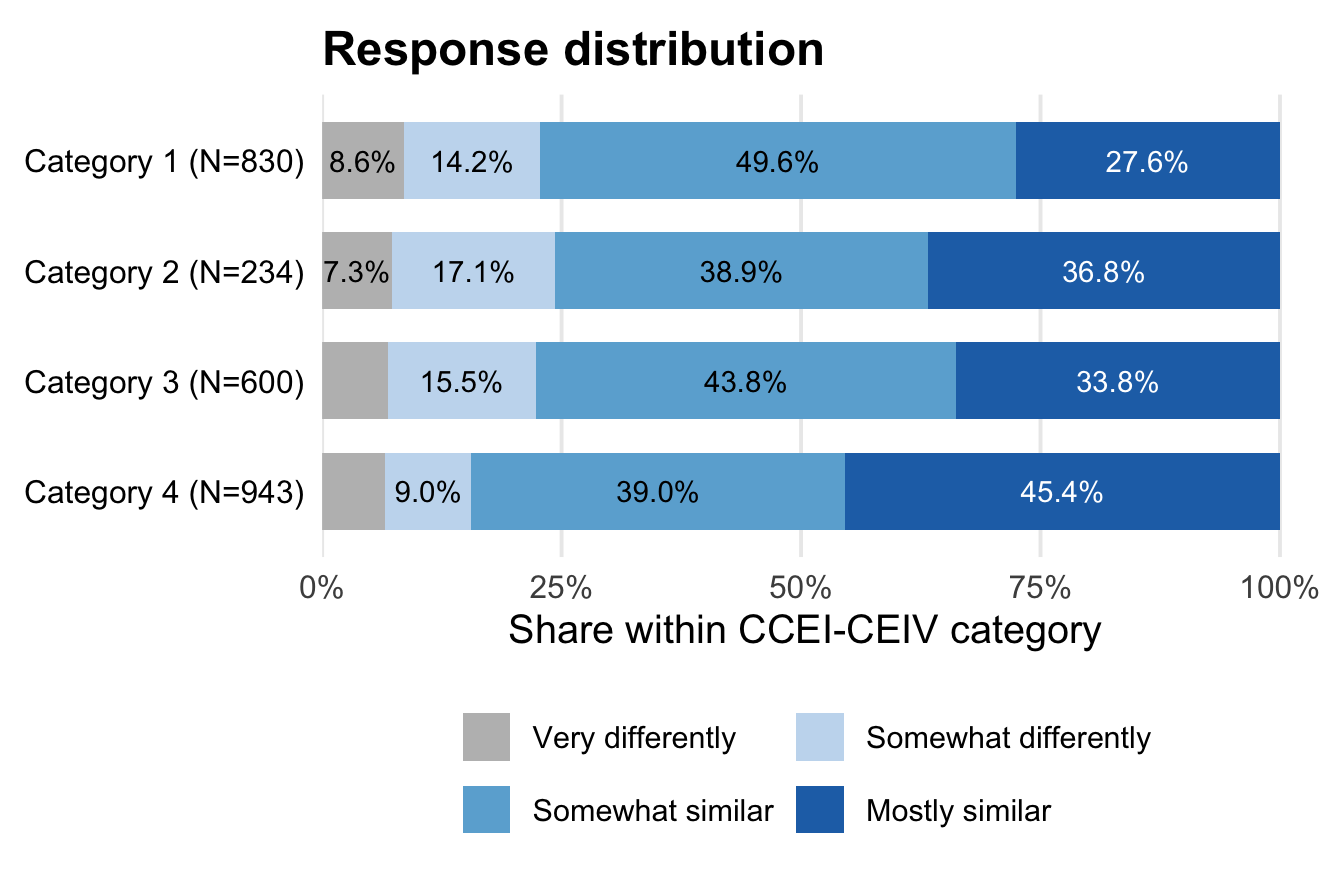
\includegraphics[width=0.595\textwidth]{similar_distribution.png}
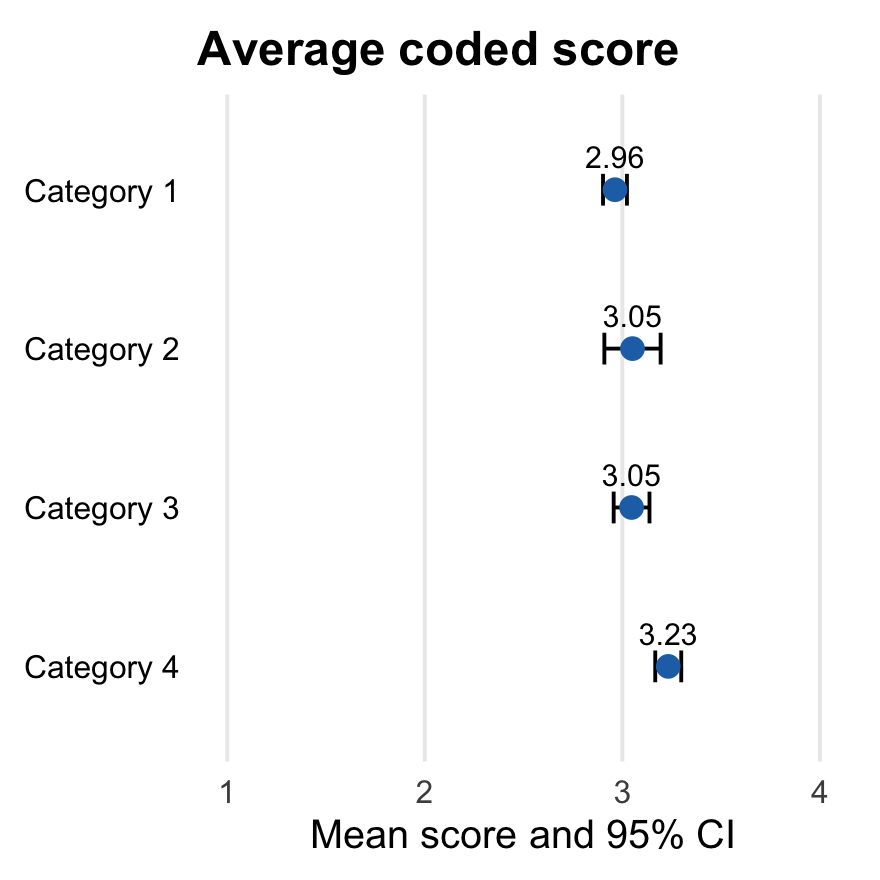
\includegraphics[width=0.395\textwidth]{similar_mean.png}
\end{center}
\small
Survey: If you had individually made decisions under the same choice environments as in the group experiment, how similar do you think those decisions would have been? Scores run from 1 (very differently) to 4 (mostly similar).

\begin{center}\begin{tabular}{clrrrr}\toprule
Category & Group outcomes & Very differently & Somewhat differently & Somewhat similar & Mostly similar\\\midrule
1 & CCEI$<1$, CEIV$<1$ & 8.6 & 14.2 & 49.6 & 27.6\\
2 & CCEI$=1$, CEIV$<1$ & 7.3 & 17.1 & 38.9 & 36.8\\
3 & CCEI$<1$, CEIV$=1$ & 6.8 & 15.5 & 43.8 & 33.8\\
4 & CCEI$=1$, CEIV$=1$ & 6.6 & 9.0 & 39.0 & 45.4\\
\bottomrule\end{tabular}\end{center}
\textit{Notes:} Table entries are percentages within each group category. Response counts are 830, 234, 600, 943. Category 4 has one missing respondent; all other responses are observed. Joint class-clustered tests of equal response distributions: all four categories, $p<0.001$; categories 4 and 3, $p<0.001$. Tests use stacked linear probability models for all but one response indicator, with unrestricted category-by-response means.
Category 4 minus category 3 in mean score: 0.186 ($p<0.001$). Mean-score intervals are 95\% t intervals using class-clustered standard errors.
\clearpage
\begin{center}\Large\textbf{Whose suggestions were reflected?}\end{center}
\begin{center}
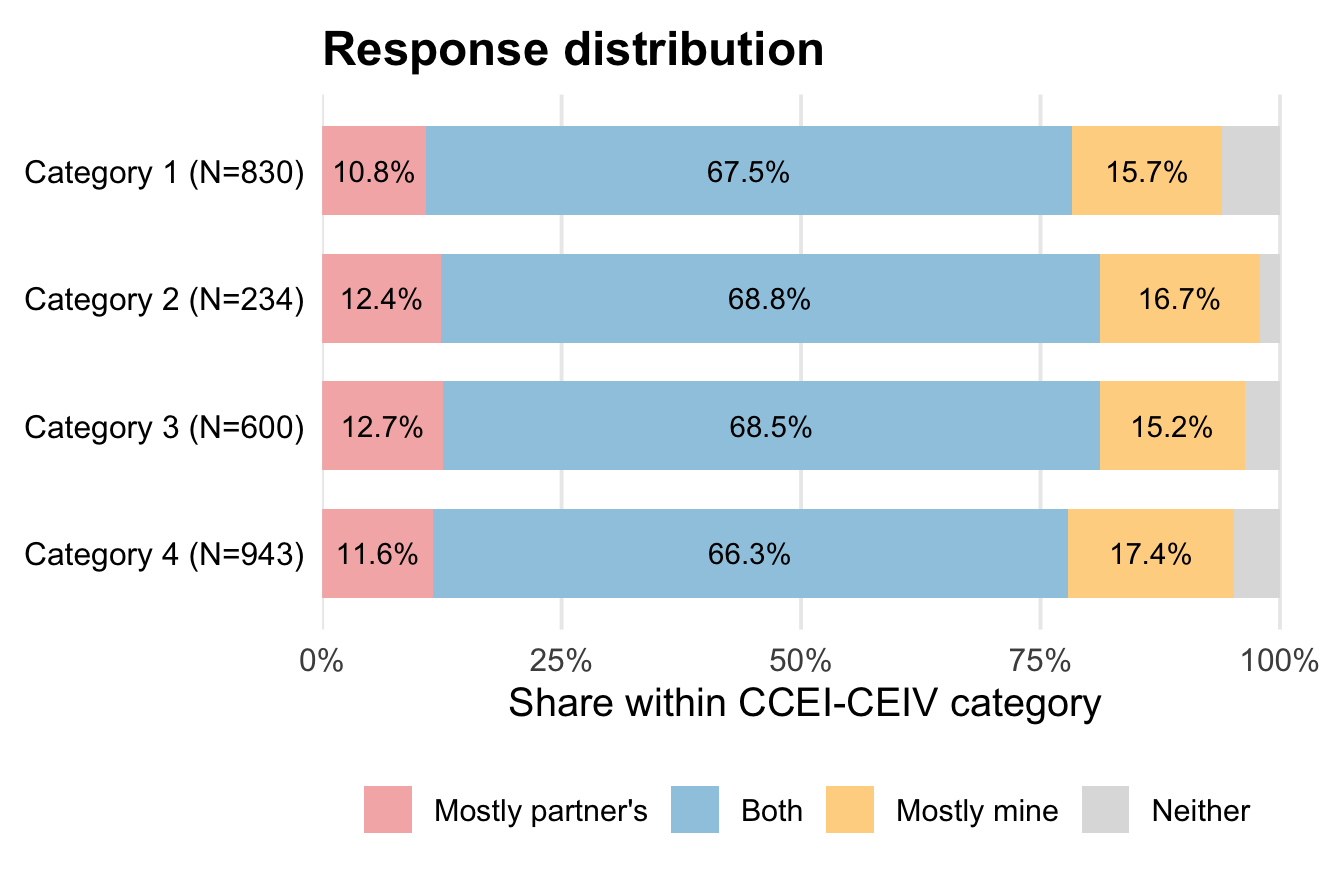
\includegraphics[width=0.58\textwidth]{whose_distribution.png}
\end{center}
\small
Survey: During the collective choice experiment, whose suggestions were most reflected in the final choices? Responses are nominal; neither their mean nor an ordinal correlation is reported.

\begin{center}\begin{tabular}{clrrrr}\toprule
Category & Group outcomes & Mostly partner's & Both & Mostly mine & Neither\\\midrule
1 & CCEI$<1$, CEIV$<1$ & 10.8 & 67.5 & 15.7 & 6.0\\
2 & CCEI$=1$, CEIV$<1$ & 12.4 & 68.8 & 16.7 & 2.1\\
3 & CCEI$<1$, CEIV$=1$ & 12.7 & 68.5 & 15.2 & 3.7\\
4 & CCEI$=1$, CEIV$=1$ & 11.6 & 66.3 & 17.4 & 4.8\\
\bottomrule\end{tabular}\end{center}
\textit{Notes:} Table entries are percentages within each group category. Response counts are 830, 234, 600, 943. Category 4 has one missing respondent; all other responses are observed. Joint class-clustered tests of equal response distributions: all four categories, $p=0.309$; categories 4 and 3, $p=0.337$. Tests use stacked linear probability models for all but one response indicator, with unrestricted category-by-response means.
``Both'' is reported by 66.3\% in category 4 and 68.5\% in category 3 ($p=0.412$); this difference is not statistically distinguishable from zero.
\clearpage
\begin{center}\Large\textbf{Risk-survey responses: less rational member only}\end{center}
\textbf{Selection.} Keep the member with strictly lower individual CCEI in each pair and wave, using a $10^{-9}$ tie tolerance.
All 199 ties are exact ties in the stored data. These pair-waves have no uniquely less rational member and are excluded:
37, 17, 31, and 114 in categories 1--4, respectively. The remaining 1,105 lower-CCEI members have observed answers to
all three questions. Ranking is wave-specific, so the selected member can change between waves. No RA-gap restriction
is applied, and group categories are defined exactly as in the preceding section.

\begin{center}\small\begin{tabular}{clrrrrr}\toprule
Category & Group outcomes & Pair-waves & Lower-CCEI members & Cooperation & Similarity & ``Both''\\
& & & with answers & Mean (1--5) & Mean (1--4) & Share (\%)\\\midrule
1 & CCEI$<1$, CEIV$<1$ & 378 & 378 & 4.354 & 2.992 & 65.1\\
2 & CCEI$=1$, CEIV$<1$ & 100 & 100 & 4.410 & 3.130 & 69.0\\
3 & CCEI$<1$, CEIV$=1$ & 269 & 269 & 4.320 & 2.970 & 68.4\\
4 & CCEI$=1$, CEIV$=1$ & 358 & 358 & 4.469 & 3.193 & 67.3\\
\bottomrule\end{tabular}\end{center}
\textbf{Relevant contrast: category 4 minus category 3.} Both categories have CEIV$=1$;
they differ in whether group CCEI also equals one. This comparison does not hold other pair characteristics fixed.
\begin{center}\small
\begin{tabular}{lrrr}\toprule
Survey measure & Difference & 95\% confidence interval & $p$\\\midrule
Cooperation score & 0.150 & [-0.011, 0.310] & 0.067\\
Similarity score & 0.222 & [0.095, 0.350] & $<0.001$\\
Both suggestions reflected (percentage points) & -1.083 & [-8.689, 6.523] & 0.777\\
\bottomrule\end{tabular}\end{center}
\small
\textbf{Reading the pattern.} Among less rational members, similarity to hypothetical own choices remains higher in
category 4 than category 3 (0.222 points, $p<0.001$). Cooperation is also higher (0.150 points), but its confidence interval
includes zero ($p=0.067$). ``Both'' suggestions being reflected shows little difference ($p=0.777$). This is consistent
with greater perceived alignment, but does not establish stable aggregation weights or a conversation about preferences.

\textit{Notes:} Descriptive, unadjusted comparisons clustered by 64 classes, without multiple-testing adjustment.
Cooperation and similarity means assume equal spacing between coded responses. The nominal whose-suggestions answers
are shown as distributions. Comparisons with the all-member section reflect both selecting the lower-CCEI member and
excluding tied pair-waves; tied pairs are disproportionately represented in category 4.
\clearpage
\begin{center}\Large\textbf{Less rational members: cooperation}\end{center}
\begin{center}
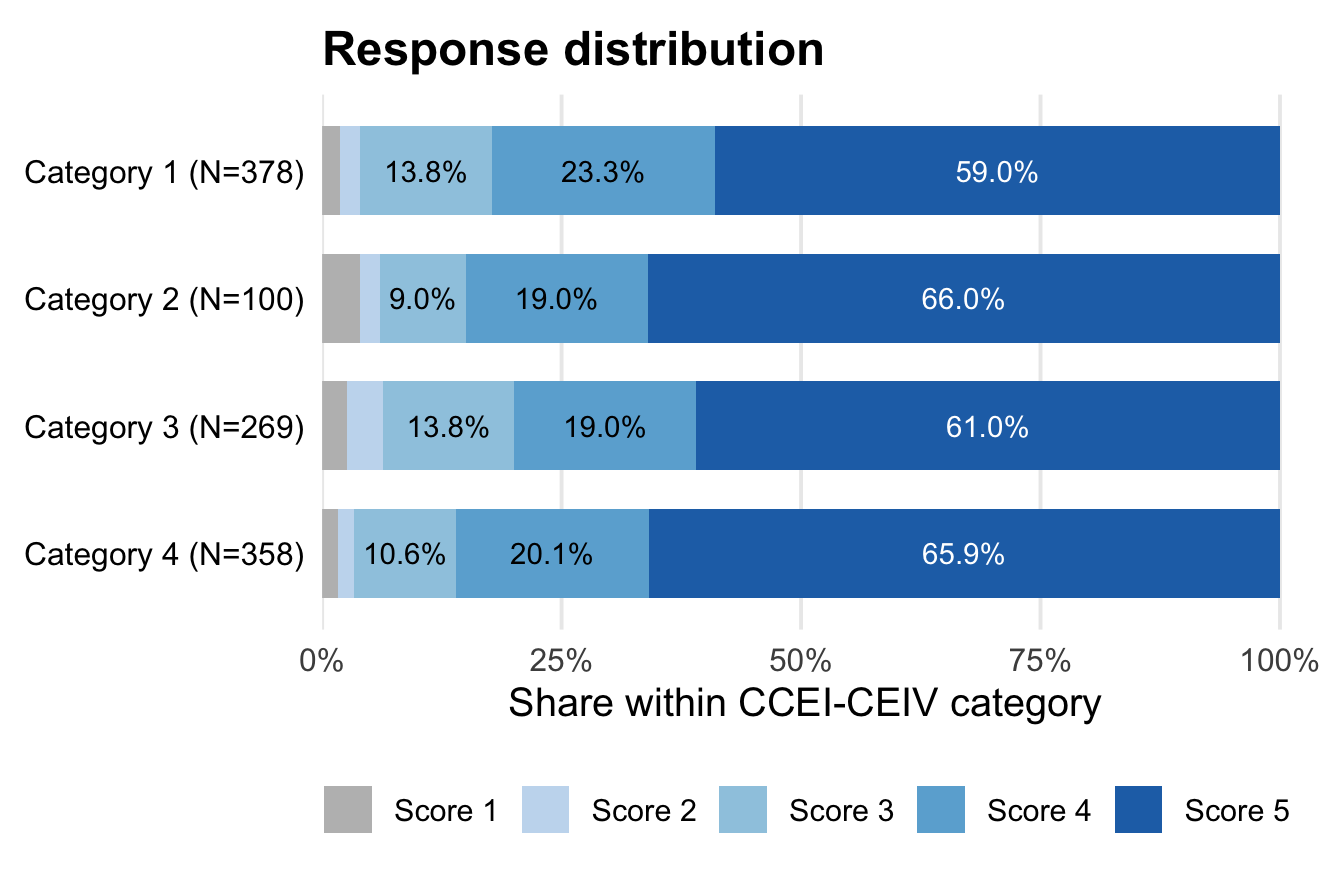
\includegraphics[width=0.595\textwidth]{less_cooperation_distribution.png}
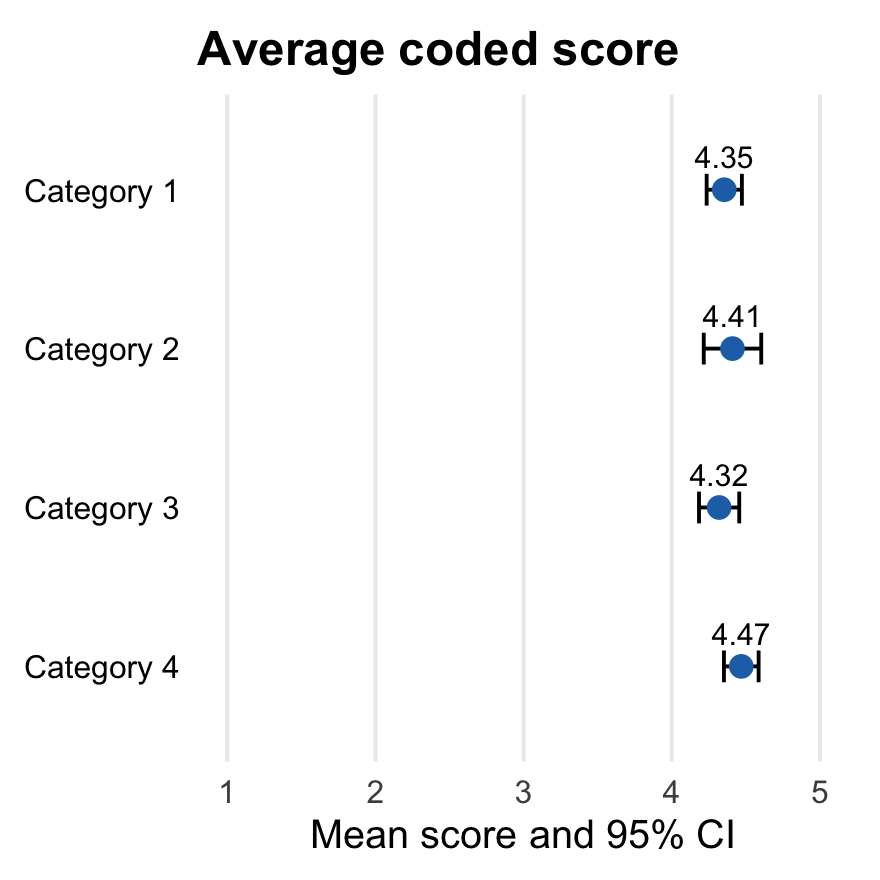
\includegraphics[width=0.395\textwidth]{less_cooperation_mean.png}
\end{center}
\small
Cooperation uses coded scores 1 to 5, with higher scores indicating greater cooperation. Exact original wording and answer anchors have not been recovered and are not reconstructed here.

\begin{center}\begin{tabular}{clrrrrr}\toprule
Category & Group outcomes & 1 & 2 & 3 & 4 & 5\\\midrule
1 & CCEI$<1$, CEIV$<1$ & 1.9 & 2.1 & 13.8 & 23.3 & 59.0\\
2 & CCEI$=1$, CEIV$<1$ & 4.0 & 2.0 & 9.0 & 19.0 & 66.0\\
3 & CCEI$<1$, CEIV$=1$ & 2.6 & 3.7 & 13.8 & 19.0 & 61.0\\
4 & CCEI$=1$, CEIV$=1$ & 1.7 & 1.7 & 10.6 & 20.1 & 65.9\\
\bottomrule\end{tabular}\end{center}
\textit{Notes:} Table entries are percentages within each group category. Response counts are 378, 100, 269, 358. One lower-CCEI member per untied pair-wave; all 1,105 selected members have observed answers. CCEI ties within $10^{-9}$ are excluded. Joint class-clustered tests of equal response distributions: all four categories, $p=0.339$; categories 4 and 3, $p=0.136$. Tests use stacked linear probability models for all but one response indicator, with unrestricted category-by-response means.
Category 4 minus category 3 in mean score: 0.150 ($p=0.067$). Mean-score intervals are 95\% t intervals using class-clustered standard errors.
\clearpage
\begin{center}\Large\textbf{Less rational members: own-choice similarity}\end{center}
\begin{center}
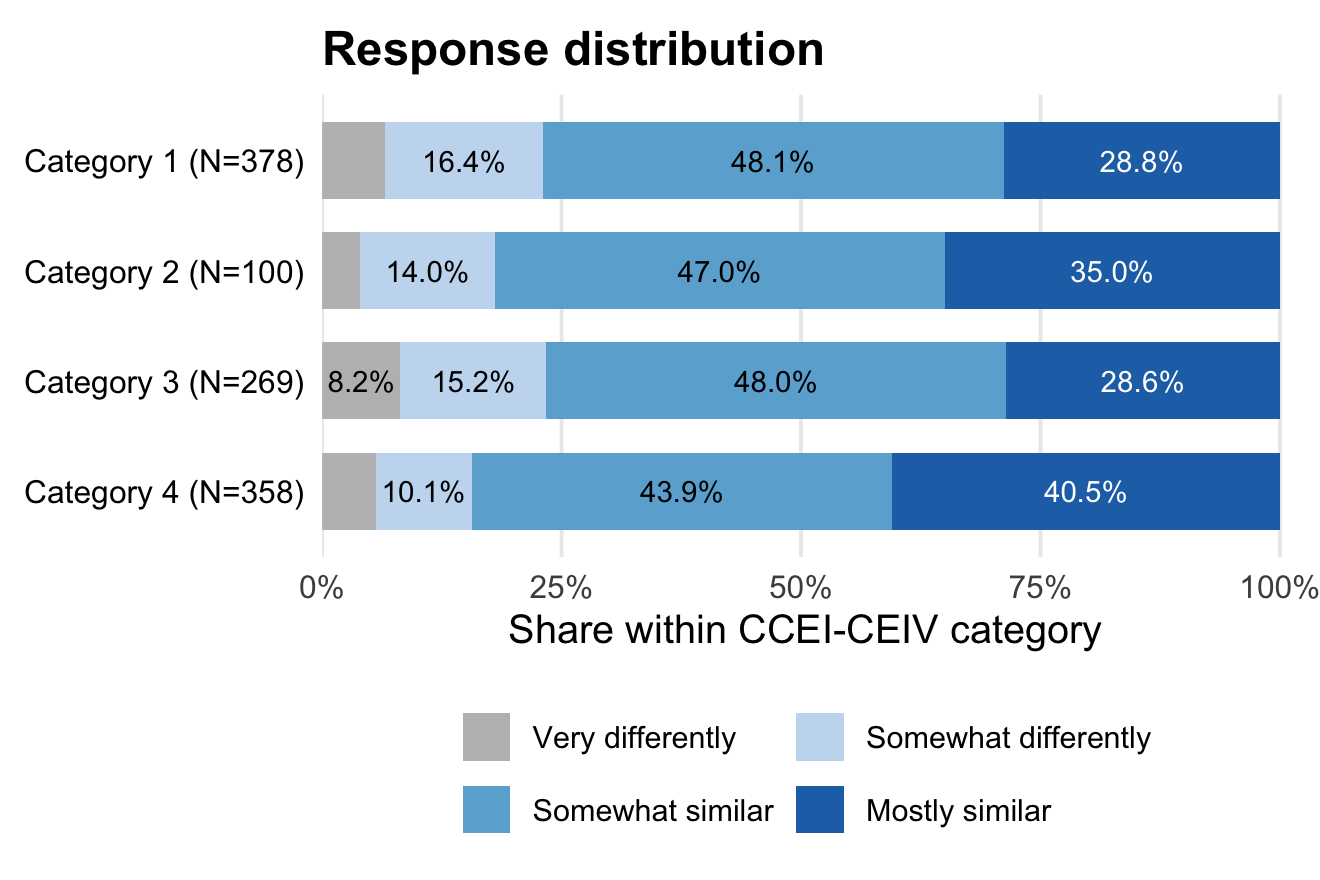
\includegraphics[width=0.595\textwidth]{less_similar_distribution.png}
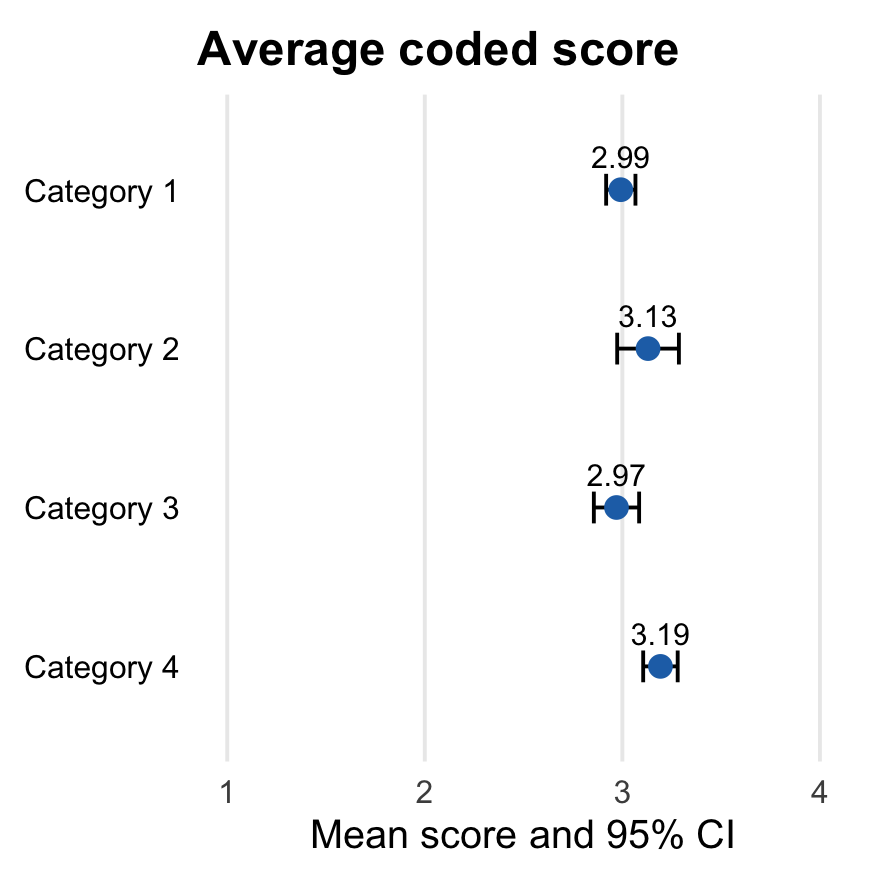
\includegraphics[width=0.395\textwidth]{less_similar_mean.png}
\end{center}
\small
Survey: If you had individually made decisions under the same choice environments as in the group experiment, how similar do you think those decisions would have been? Scores run from 1 (very differently) to 4 (mostly similar).

\begin{center}\begin{tabular}{clrrrr}\toprule
Category & Group outcomes & Very differently & Somewhat differently & Somewhat similar & Mostly similar\\\midrule
1 & CCEI$<1$, CEIV$<1$ & 6.6 & 16.4 & 48.1 & 28.8\\
2 & CCEI$=1$, CEIV$<1$ & 4.0 & 14.0 & 47.0 & 35.0\\
3 & CCEI$<1$, CEIV$=1$ & 8.2 & 15.2 & 48.0 & 28.6\\
4 & CCEI$=1$, CEIV$=1$ & 5.6 & 10.1 & 43.9 & 40.5\\
\bottomrule\end{tabular}\end{center}
\textit{Notes:} Table entries are percentages within each group category. Response counts are 378, 100, 269, 358. One lower-CCEI member per untied pair-wave; all 1,105 selected members have observed answers. CCEI ties within $10^{-9}$ are excluded. Joint class-clustered tests of equal response distributions: all four categories, $p=0.015$; categories 4 and 3, $p=0.009$. Tests use stacked linear probability models for all but one response indicator, with unrestricted category-by-response means.
Category 4 minus category 3 in mean score: 0.222 ($p<0.001$). Mean-score intervals are 95\% t intervals using class-clustered standard errors.
\clearpage
\begin{center}\Large\textbf{Less rational members: whose suggestions?}\end{center}
\begin{center}
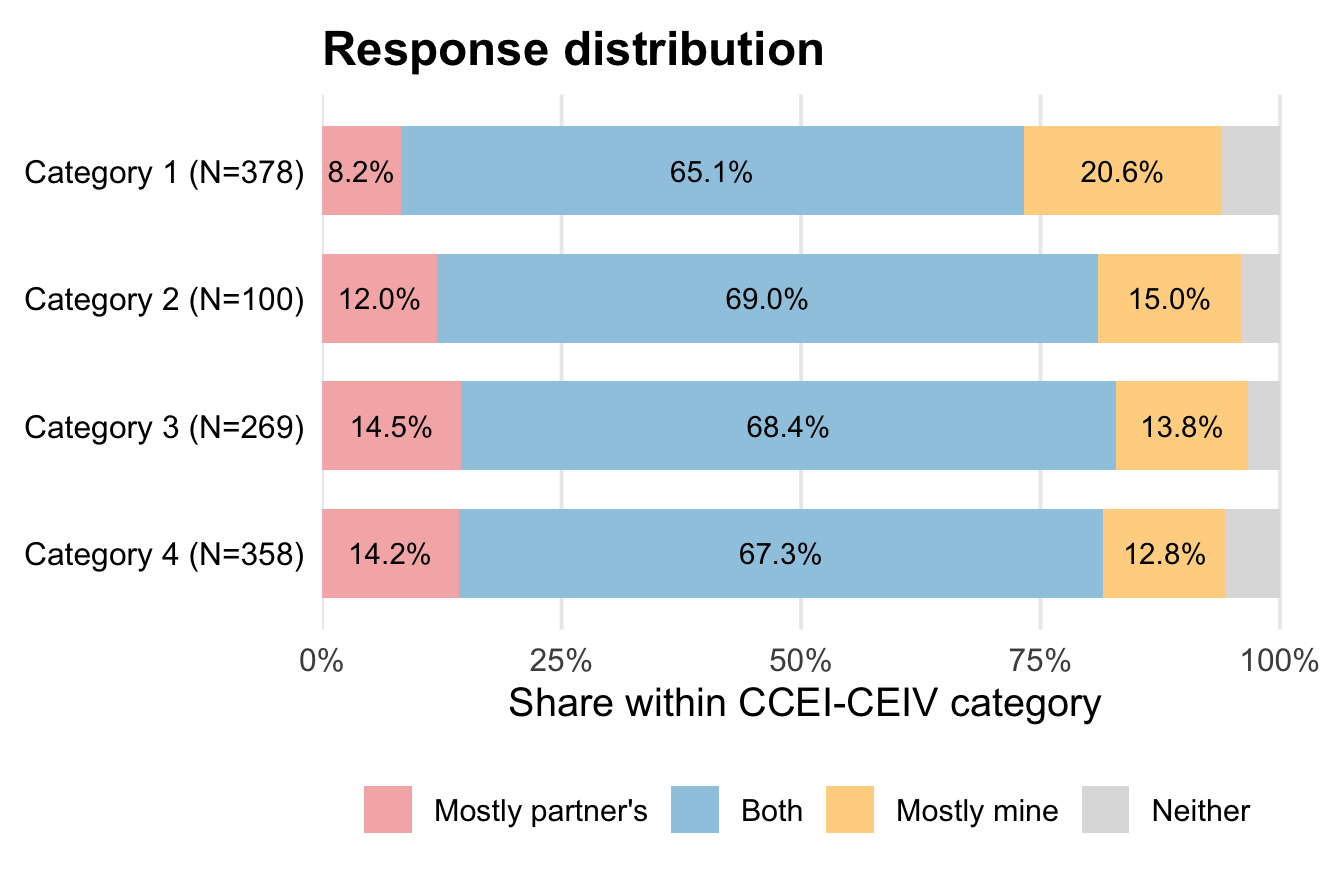
\includegraphics[width=0.58\textwidth]{less_whose_distribution.png}
\end{center}
\small
Survey: During the collective choice experiment, whose suggestions were most reflected in the final choices? Responses are nominal; neither their mean nor an ordinal correlation is reported.

\begin{center}\begin{tabular}{clrrrr}\toprule
Category & Group outcomes & Mostly partner's & Both & Mostly mine & Neither\\\midrule
1 & CCEI$<1$, CEIV$<1$ & 8.2 & 65.1 & 20.6 & 6.1\\
2 & CCEI$=1$, CEIV$<1$ & 12.0 & 69.0 & 15.0 & 4.0\\
3 & CCEI$<1$, CEIV$=1$ & 14.5 & 68.4 & 13.8 & 3.3\\
4 & CCEI$=1$, CEIV$=1$ & 14.2 & 67.3 & 12.8 & 5.6\\
\bottomrule\end{tabular}\end{center}
\textit{Notes:} Table entries are percentages within each group category. Response counts are 378, 100, 269, 358. One lower-CCEI member per untied pair-wave; all 1,105 selected members have observed answers. CCEI ties within $10^{-9}$ are excluded. Joint class-clustered tests of equal response distributions: all four categories, $p=0.059$; categories 4 and 3, $p=0.637$. Tests use stacked linear probability models for all but one response indicator, with unrestricted category-by-response means.
``Both'' is reported by 67.3\% in category 4 and 68.4\% in category 3 ($p=0.777$); this difference is not statistically distinguishable from zero.
\end{document}
